\documentclass{beamer}
\usepackage[francais]{babel}
\usepackage[T1]{fontenc}
\usepackage[utf8]{inputenc}  
\usepackage{verbatim} 
\usepackage{indentfirst}          %pour \verbatiminput{fich}
\usetheme{JuanLesPins}    % titre en haut
\useoutertheme{default}       
\setlength{\parindent}{0.5cm}

\graphicspath{{Figures/}}
\setbeamertemplate{caption}[numbered] % pour numéroter tables et figures !
%si \verb   : \begin{frame}[fragile]
%si verbatim  : \begin{frame}[containsverbatim]


\title{SudokuSolver}
\author{Jérémy SIMIONE, Thomas BESSON , Leif HENRIKSEN}
\institute{Université de Montpellier}
\date{2019}

\begin{document}
% Premier transparent de titre
\begin{frame}
  \titlepage
\end{frame}

% 2eme transparent TDM générale
\AtBeginSection[]
{
    \begin{frame}
        \frametitle{Sommaire}
        \tableofcontents[currentsection,hideothersubsections]
    \end{frame}
}

\section{Sudoku création}
\subsection{Définition}
\begin{frame}
\frametitle{Définition}

\begin{figure}
        \centering
        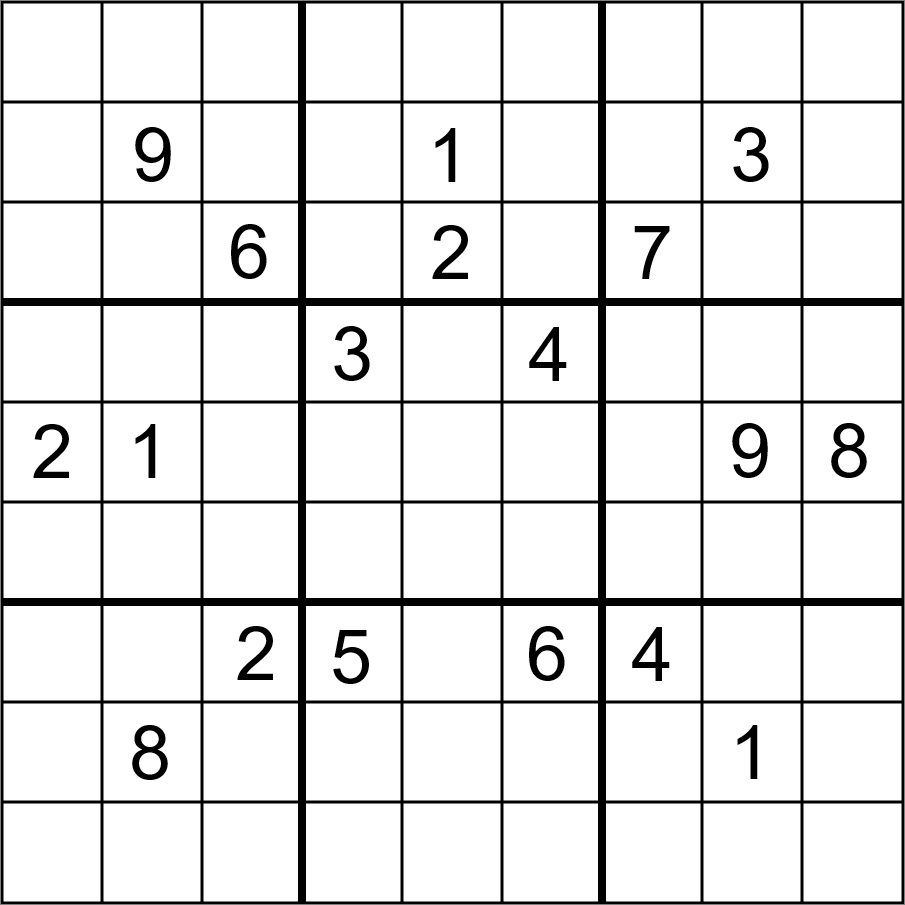
\includegraphics[width=150]{img/sud.png}
        \caption{Sudoku}
        \label{fig:my_label}
    \end{figure}
    
\end{frame}

\begin{frame}

\subsection{L'idée du projet}
\frametitle{Projet}
\begin{itemize}
    \item Créer une application sur Android pour résoudre des sudokus.
    \item Le point important de ce projet était la reconnaissance de grille.

     \begin{figure}[htbp]
        
\includegraphics[width=100]{img/open.png}
        \caption{Reconnaisance d'image}
        \label{fig:my_label}
    \end{figure}
    
\end{itemize}
\end{frame}


\begin{frame}

\subsection{Création de l'application}
\frametitle{Outils}
\begin{figure}
        \centering
        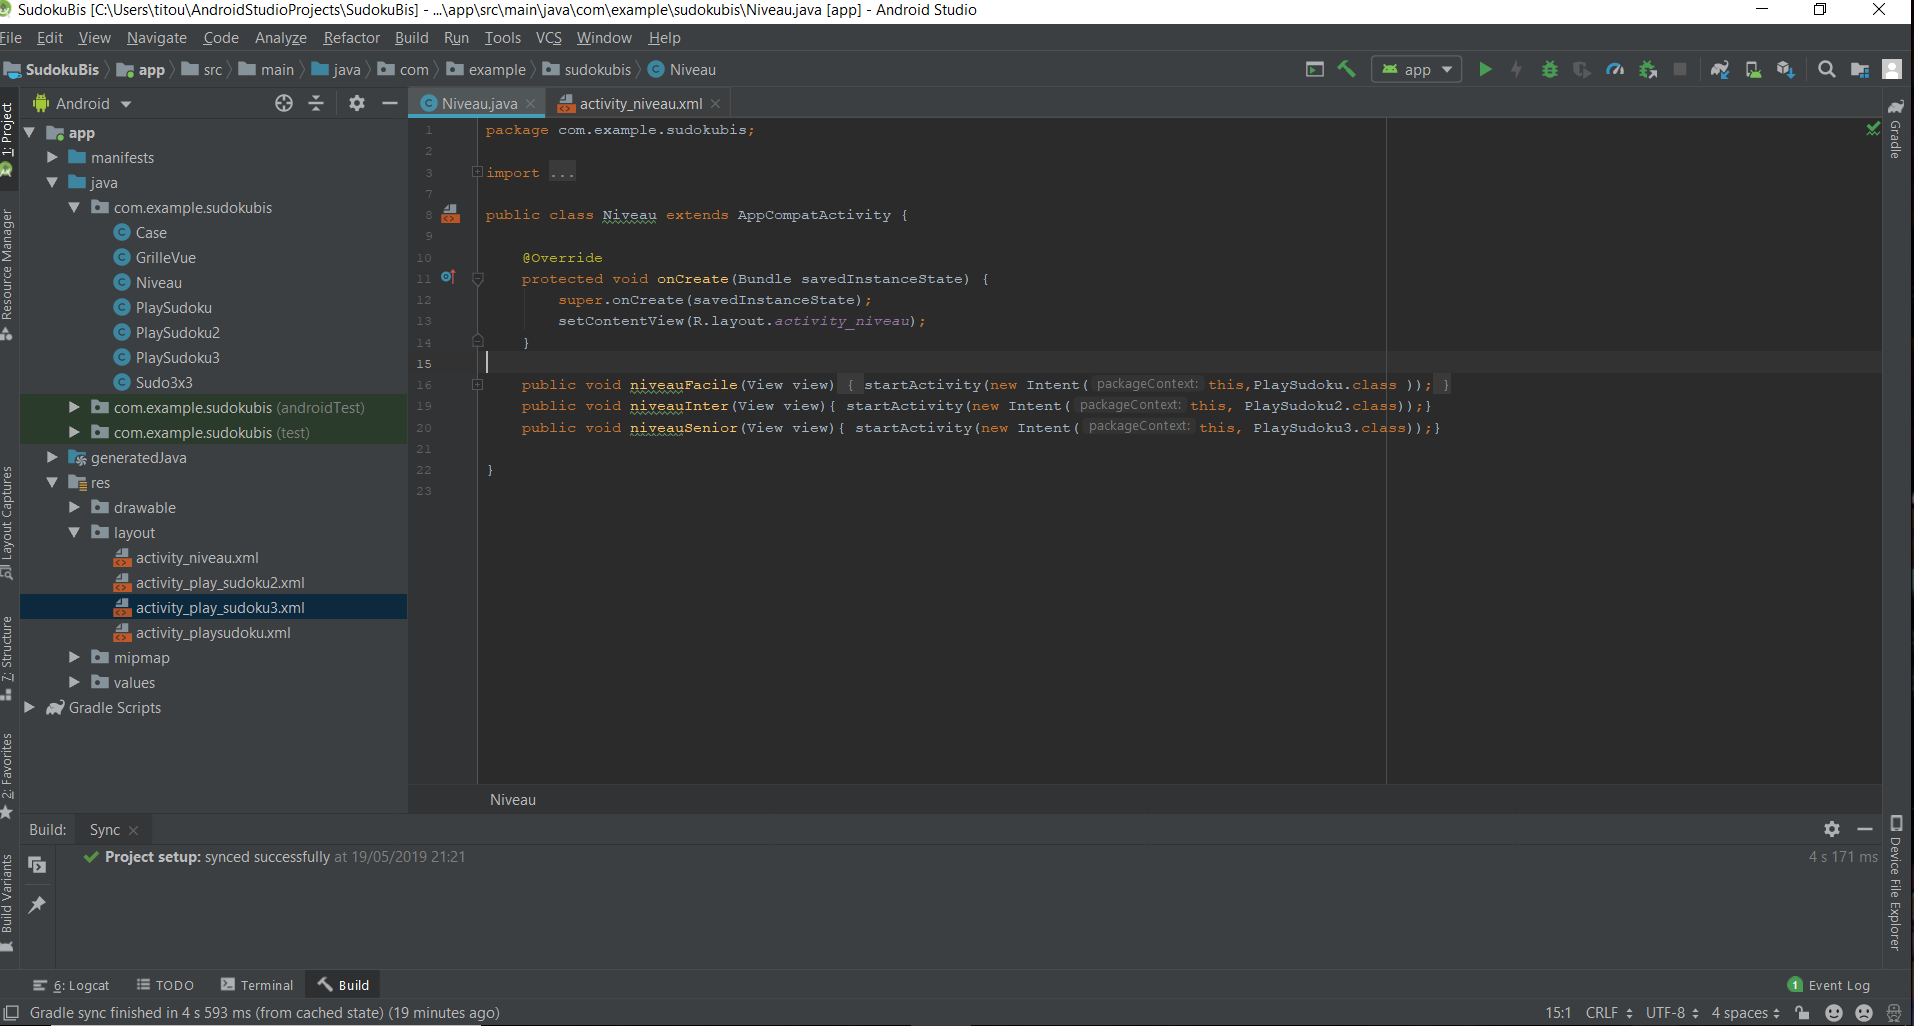
\includegraphics[width=300]{img/andro.png}
        \caption{Android Studio}
        \label{fig:my_label}
    \end{figure}

 
\end{frame}

\end{document} 